\noindent
{\bf Collaborative research: Self-organization modeled by moving domain
elliptic PDEs} \\
{Bryan Quaife (lead PI, Florida State University), \em Rolf Ryham (PI,
Fordham University), and Yuan-Nan Young (PI, New Jersey Institute of
Technology)}

\section{Background}
\label{sec:background}

The field of self-organization encompasses a broad range of interesting
and challenging phenomena in engineering and science. For example,
understanding the organization of lipids and proteins in vesicles is
crucial to designing effective drug carriers and functional mimics of
cells~\cite{Marui2022IncreasedEO,
https://doi.org/10.1002/adma.202206288}. The COVID-19 pandemic has led
to a concerted effort to understand the mechanisms of RNA condensation
by structural proteins that control virus
structure~\cite{Kim2021SelfassembledMV}. Engineers have developed
superior techniques that rely on nanoscale capillary and van der Waals
forces to print high-resolution features on
devices~\cite{Zeng20223DprintedMT}. Finally, researchers design
efficient algorithms for constructing interaction kernels in the to
study of agent-based systems like swarms and
flocking~\cite{Lu2019NonparametricIO, Tadmor2021OnTM}.

%A number of mathematical techniques have been developed to handle
%self-organizing systems. Each technique has its advantages and
%disadvantages. Prominent in chemistry and biology, molecular dynamics
%(MD) simulations offers unparalleled resolution of protein-lipid
%interactions, say, but because of the large number of non-linear
%interactions involved, is limited to short time and small spatial
%scales. In terms of inverse problems, agent based systems also involve
%relatively large numbers of particles and researchers extensively
%consider the problem of using trajectory data to learn interaction
%kernels of the dynamics when constrained to evolve on Riemannian
%manifolds. Once the interaction kernels are known, one can in principle
%derive partial differential equations (PDE) for the macroscopic
%behavior. 

When fluids are involved, tracking self-organization becomes difficult
due to the deformability of suspended media in the presence of non-local
hydrodynamic interactions. The phase field method, a prominent approach
in this area, introduces a scalar-valued phase field function for the
volume fraction of amphiphilic lipids or polymers in solvent, for
example. Sometimes called the diffuse interface method, one devises
energy functionals involving the gradient and well-potentials of the
phase field, and possibly convolution kernels, to characterize the self-
and solvent-interaction of the suspended
media~\cite{Promislow2022UndulatedBI, C9SM01983A,doi:10.1063/5.0009734,
LiAn-Chang16, Choksi2003OnTD}. Because the fluid interfaces are given by
level-sets of a smooth function, they can have almost arbitrary topology
e.g., free ends, junctions~\cite{Promislow2017ExistenceBA,
Promislow2022UndulatedBI}, the evolution equations can be studied by
well-established variational and analytical
tools~\cite{Gavish2011CurvatureDF, Dai2019WeakSF, Dai2015CompetitiveGE,
Dai2022GeometricEO, Dai2020MinimizersFT, Dai2013GeometricEO}, and the
governing equations are amenable to numerical
approximation~\cite{Christlieb2020BenchmarkCO,
Christlieb2019CompetitionAC}. One of the downsides, though, is that
granular details like molecular heterogeneity and orientations that may
be crucial to the physics at mesoscopic scales \cite{Midya2022}, are blurred
by the model. Moreover, numerical simulations of phase field
models typically discretize the entire fluid domain, and apply cutoff
boundary conditions when periodic domains are not under consideration. 

The PIs recently developed a new mathematical model of self-organization
in fluid systems~\cite{FuQuRyYo22, fu-ryh-qua-you2022, Fu2018_SIAM}. The
framework uses small, rigid bodies called ``granules'' to represent
parcels of suspended media. The granule shapes and boundary conditions
capture the local properties of the suspension, and instead of volume
fraction, a phase field function represents the properties of the
solvent. Our approach falls into the category of work that considers
particles as a discretization of a continuous problem; in this case one
is dealing with a particle method, as an alternative to other
stencil-based discretization methods~\cite{Wilson2021ComparisonOT,Gross2020MeshfreeMO,
Sigurdsson2016HydrodynamicCO}.
We have departed from the terminology ``particles'', though,
to emphasize the role played elliptic equations and the granules'
finite size.

The framework is robust, flexible, and cuts across many of the
aforementioned challenges. (i) The granules are not fixed to a stencil,
affording flexibility in terms of morphology and topology---sufficiently
large forces will even pull groups of granules apart as physically
required. (ii) The model formulation is built around important details
like molecular orientations, and exhibits inter-molecular slip that must
be added into continuum models post hoc. (iii) It is
straightforward to consider mixtures of granules with different shapes
and boundary conditions. Leveraging boundary integral and fast summation
methods, the dynamics can be solved in near-linear complexity in the
number of granules, which is equal to or better than the computational
complexity of related sharp interface methods. 

\begin{figure}
  \begin{center}
    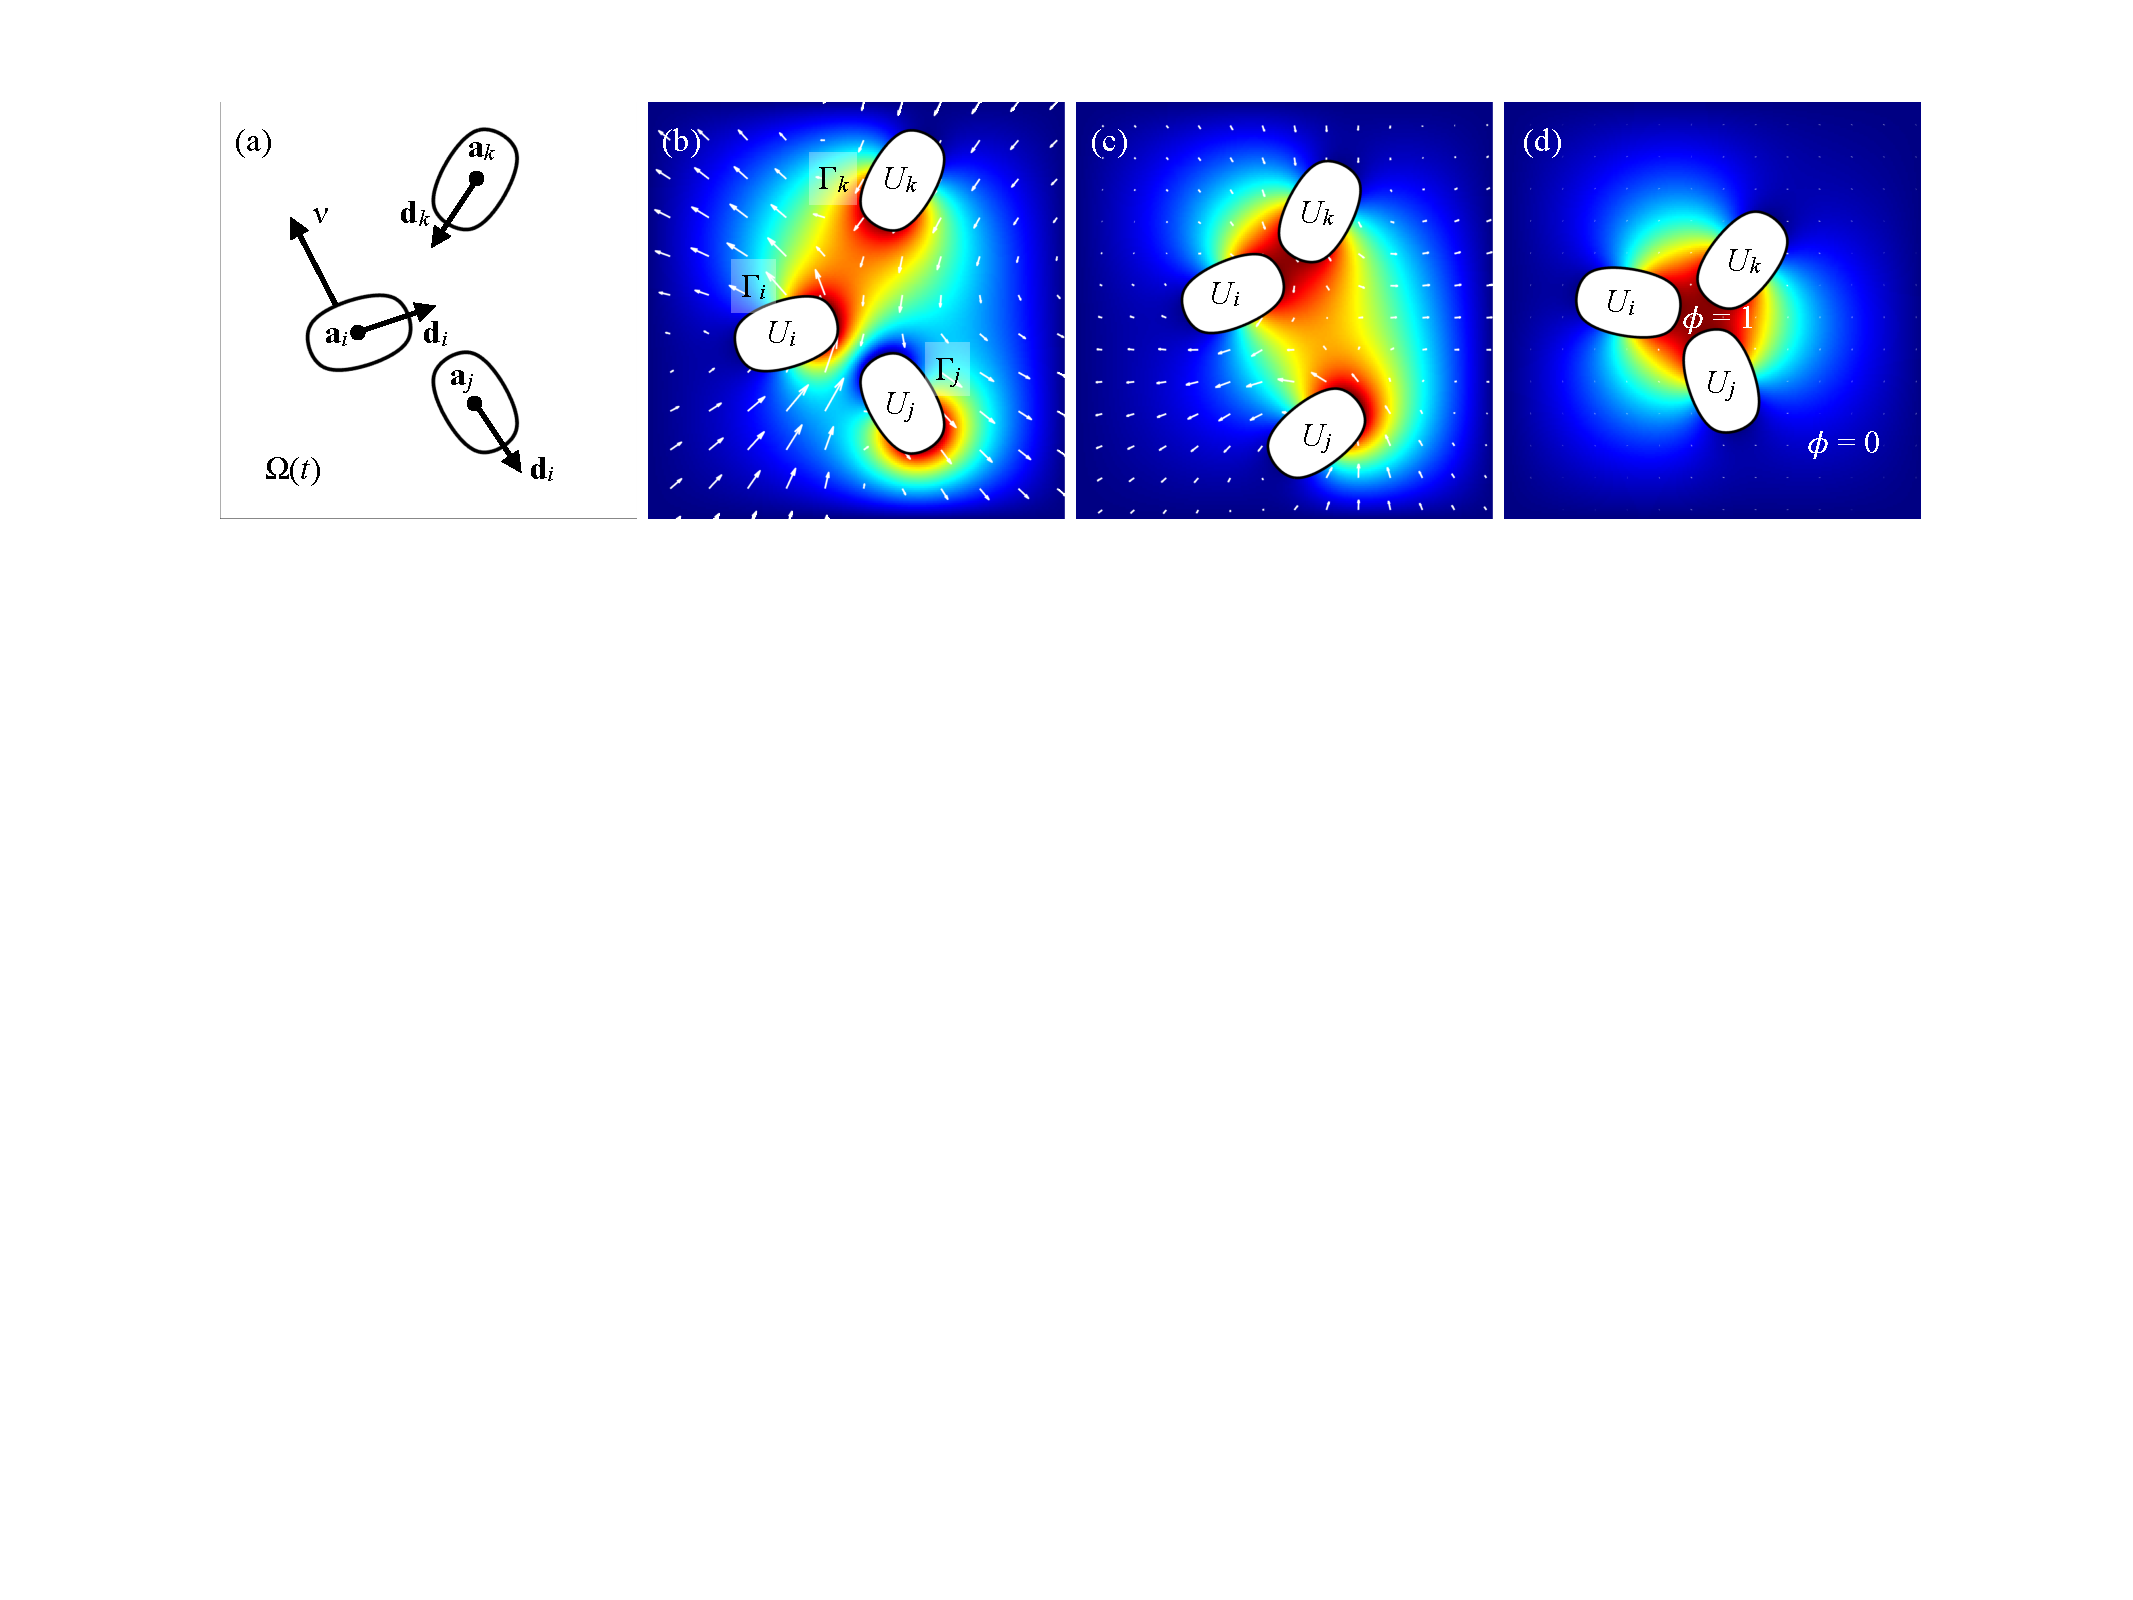
\includegraphics[width=\textwidth]{figures/Background/Domain.pdf}
%    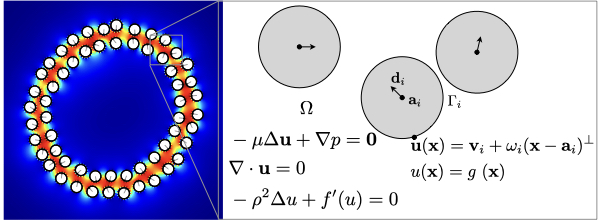
\includegraphics[width=0.45\textwidth]{figures/SpecificAim1/Domain.jpg}
%    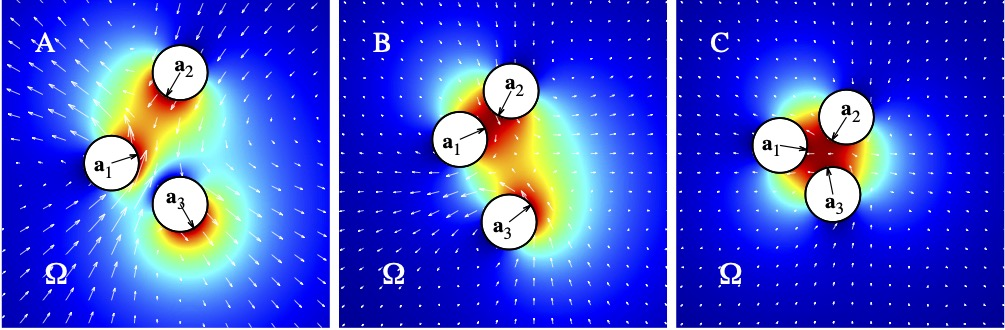
\includegraphics[width=0.45\textwidth]{figures/SpecificAim1/3Particles.jpg}
%    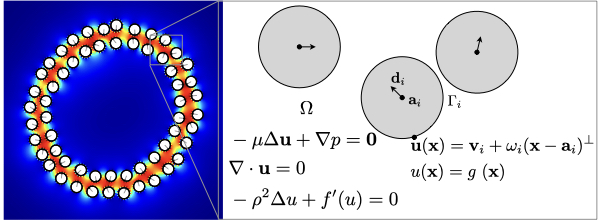
\includegraphics[keepaspectratio,height=2.7cm]{figures/SpecificAim1/Domain.jpg}
%    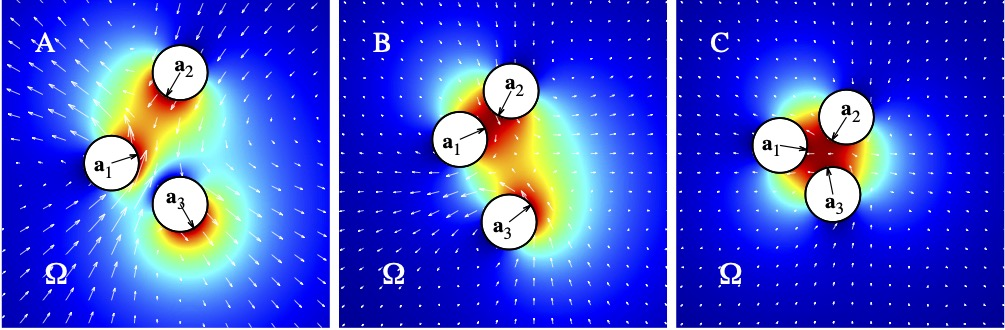
\includegraphics[keepaspectratio,height=2.7cm]{figures/SpecificAim1/3Particles.jpg}
  \end{center}
  \caption{\label{fig:flow_map} \footnotesize (a) Granules make a
  superstructure e.g., a vesicle. The panel shows the moving domain
  $\Omega(t)$, granules with centers $\aa_i$ and directors $\dd_i$, and
  the unit inward normal $\nnu$. Panels (b), (c), (d) show the interplay
  between the phase field $\phi$ (colormap) and granule configuration.
  Red is for $\phi = 1$ and blue for $\phi = 0$; $W(\phi) =
  \tfrac{1}{2}\phi^2$. The white arrows are the fluid velocity field.
  The panels reach an equilibrium state in panel (d).}
\end{figure}

\subsection{Problem formulation}
To formulate the problem, consider a collection of $N_b$-many rigid
bodies $U_i(t) \subset \RR^n$ with boundary $\Gamma_i(t)$. We call these
bodies ``granules''. The granules are immersed in an incompressible,
zero-Reynolds number fluid $\Omega(t) = \RR^n \setminus \cup_{i=1}^{N_b}
U_i(t)$ (Figure~\ref{fig:flow_map}). Throughout, $\nnu$ refers to
the unit normal pointing into $\Omega(t)$.

To determine how the granules move through space, we look for rigid body
transformations
\begin{align}
\label{eq:RBT}
  \FF_i(\XX,t) = R_i(t)(\XX - \aa_i(0)) + \aa_i(t),\quad \XX \in U_i(0),
\end{align}
where $i = 1,\ldots,N_b,$ $R_i(t)$ is an $n
\times n$ rotation matrix, $\aa_i(t)$ are the granule centers, and $\XX$ is a
reference coordinate.
The dynamics come from the following system of semi-linear, elliptic boundary value problems:
\begin{alignat}{4}
  \label{eqn:stokes} 
  -\mu\Delta \uu + \nabla p &= \mathbf{0}, 
  \quad \nabla \cdot \uu = 0, &&\xx \in \Omega(t), \\
  \label{eqn:phase}
  -\epsilon^2 \Delta \phi + W'(\phi) &= 0, &&\xx \in \Omega(t),\\
  \label{eqn:noslip}        
  \frac{d\FF_i}{dt}(\XX,t) & = \uu(\xx) = 
    \vv_i + \oomega_i \times (\xx - \aa_i), 
  \quad &&\xx \in \Gamma_i(t),\\
  \label{eqn:material}
  \phi(\xx) &= h_i(\XX),  &&\xx \in \Gamma_i(t),
\end{alignat}
for $i=1,\ldots,N_b$ and where $\xx = \FF_i(\XX,t)$. Finally,
\begin{align}
\label{eqn:stressbalance}
\int_{\Gamma_i} \left(\sigma  + T_i\right)\nnu \,\dif s = \mathbf{0},\quad
\int_{\Gamma_i} (\xx - \aa_i)\times \left(\sigma + T_i\right) \nnu
  \,\dif s = \mathbf{0},
\end{align}
where
\begin{align}
\label{eqn:hydro_stress}
\sigma = \mu(\nabla \uu + \nabla \uu^T) - pI,\quad 
T_i = \gamma\left[\epsilon^{-1} W(\phi)I
  + \epsilon\left(\tfrac{1}{2}|\nabla \phi|^2I - \nabla \phi \nabla
  \phi^T\right)\right]
\end{align}
are the hydrodynamic and phase field stresses, respectively.
Equations~\eqref{eqn:stokes} are the Stokes equations describing the
velocity $\uu$ and pressure $p$ of the incompressible fluid region with
viscosity $\mu$. Equation~\eqref{eqn:phase} describes the transitions
of the scalar order parameter $\phi$ with a decay length $\epsilon$.
The scalar function $W(\phi) : \RR \to \RR$ is a nonnegative
well-potential with local minima $\phi_0, \phi_1$, etc., representing
metastable states of the solvent. In the single-well case, $W(\phi) =
\frac{1}{2}\phi^2$ has the minimum $\phi_0 = 0$ and the phase field
equation~\eqref{eqn:phase} becomes the \emph{linear} screened Laplace
equation. In the double-well case e.g, $W(\phi) =
\frac{1}{4}(\phi^2-1)^2+cx$, $c > 0$, the phase field
equation~\eqref{eqn:phase} takes the form of an Allen-Cahn equation with
local minima $\phi_0 < 0 < \phi_1$. Section \ref{sec:specificaim1}
discusses certain modifications needed for~\eqref{eqn:phase} in the
nonlinear case.

\begin{wrapfigure}[21]{r}{3.2in}
  \vspace{-15pt}
  \begin{center}
    \begin{tabular}{m{0.9in}m{0.9in}m{0.9in}}                 
    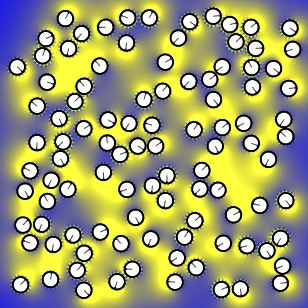
\includegraphics[width=0.85in]{figures/SpecificAim1/N100B1.jpg}
    &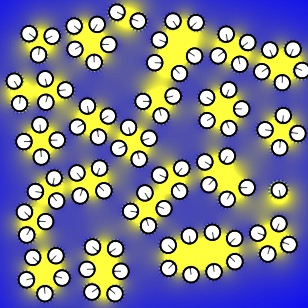
\includegraphics[width=0.85in]{figures/SpecificAim1/N100B2.jpg}
     &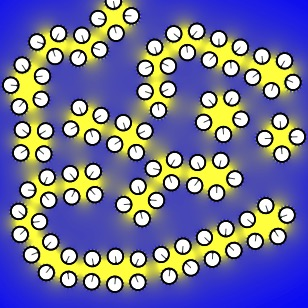
\includegraphics[width=0.85in]{figures/SpecificAim1/N100B3.jpg}    \\
    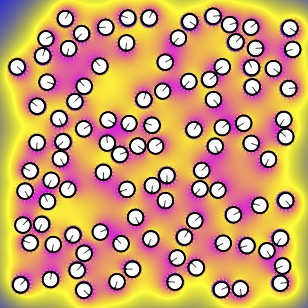
\includegraphics[width=0.85in]{figures/SpecificAim1/N100C1.jpg}
    &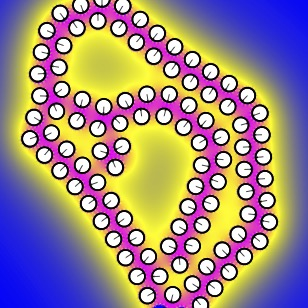
\includegraphics[width=0.85in]{figures/SpecificAim1/N100C2.jpg}
      &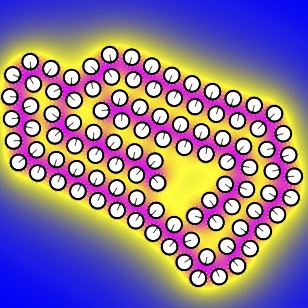
\includegraphics[width=0.85in]{figures/SpecificAim1/N100C3.jpg}    \\
      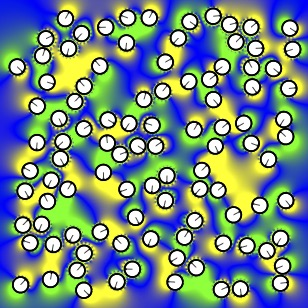
\includegraphics[width=0.85in]{figures/SpecificAim1/N100A1.jpg}
      &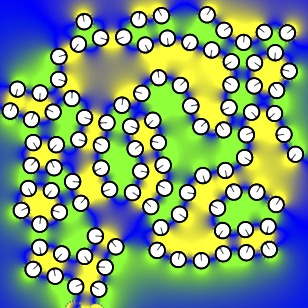
\includegraphics[width=0.85in]{figures/SpecificAim1/N100A2.jpg}
      &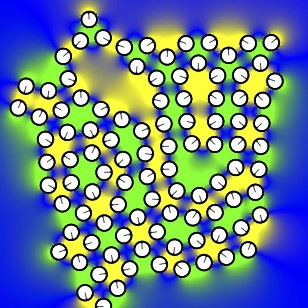
\includegraphics[width=0.85in]{figures/SpecificAim1/N100A3.jpg} 
  \end{tabular}
  \end{center}
  \vspace{-20pt}
  \caption{\footnotesize \label{fig:self-assembly2} Changes in the
  boundary condition \eqref{eqn:material} yield distinct morphologies.
  Each row has the same initial configuration; $W(\phi) =
  \tfrac{1}{2}\phi^2$. (\emph{Top}) Granules with an amphiphilic
  boundary condition form bilayer configurations (yellow, $\phi = 1$,
  blue, $\phi = 0$). (\emph{Middle}) Granules with $\phi = 2$ (magenta)
  on one side and $\phi = 1$ on the other form multilamellar bilayers.
  (\emph{Bottom}) Bipolar granules with $\phi = 1$ (yellow) on one side
  and $\phi=-1$ (green) on the other side form a checkerboard pattern.}
\end{wrapfigure}

For the moving domain, equations~\eqref{eqn:noslip}
specify a no-slip boundary condition for a rigid body with translation
velocity $\aa'_i(t) = \vv_i$ and angular velocity $\oomega_i$ (the axial
vector for $R'_i(t)R_i(t)^T$) about the point $\aa_i(t) \in U_i(t)$. In
equation~\eqref{eqn:material}, the function $h_i$ is a material label
specifying the phase at the solvent-granule interface. Finally,
equation~\eqref{eqn:stressbalance} closes the system by requiring that
the force and torque generated by hydrodynamic stress balance
the force and torque 
generated by phase stress $T_i$ in~\eqref{eqn:hydro_stress}. The
parameter $\gamma > 0$ is surface tension, $I$ is the identity matrix,
and we interpret the ``cross product'' as $\aa \times \bb = (\aa^{\perp} \cdot
\bb) \kk$ where $\kk = (0,0,1) \in \RR^3$ and $(a_1,a_2)^{\perp} =
(-a_2,a_1)$ whenever $\aa, \bb \in \mathbb{R}^2$.

\subsection{Applications}
Since the framework is scale independent, it can be applied to a broad
range of nonspecific self-organization phenomena in surface chemistry,
biology, and engineering. For one, the
formulation~\eqref{eq:RBT}--\eqref{eqn:stressbalance} captures exactly
the right behavior expected from amphiphilic self-assembly. For example,
three bodies with amphiphilic label (\S\ref{sec:specificaim1}, equation
\eqref{eq:amphiphilic_BC}) spontaneously self-organize to sequester the
hydrophobic fluid phase (Figure~\ref{fig:flow_map}). Changes in the
boundary conditions result in distinct morphologies
(Figure~\ref{fig:self-assembly2}) whose rheology can be further
investigated (\S\ref{sec:specificaim3}).
%
A concrete application the PIs have considered in their SIAM Multiscale
Modeling and Simulation and Journal of Fluid Mechanics
works~\cite{Fu2018_SIAM, FuQuRyYo22} is the problem of \emph{vesicle
hydrodynamics}.
%A vesicle is a small, fluid filled membrane sack.
The
goal in vesicle hydrodynamics is to study flow patterns arising from the
interaction between membrane elasticity/viscoelasticity and the fluid
\cite{Gera2022SwingingAT,Cox2015TheEO,wangthesis,C6SM02452A,Strychalski2012ViscoelasticIB}.


\begin{wrapfigure}[10]{l}{0.5\textwidth}
\vspace{-5pt}
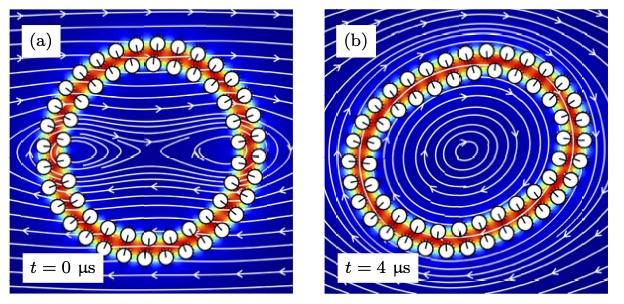
\includegraphics[width=0.5\textwidth]{figures/PreliminaryWork/TankTreading.jpg}
\vspace{-20pt}
\caption{\label{fig:JPv_linearshear} \footnotesize Granular vesicles
  undergo tank-treading in background shear flow.}
\end{wrapfigure}
%
A striking feature of our hydrodynamic simulations is their fidelity to
physics. The model contains a few parameters; granule radius $c$, decay
length $\epsilon$, surface tension $\gamma$. When these are set to
realistic values \cite{Fu2018_SIAM, ErLjCl89, Lin2005, Parsegian,
Israelachvili80, GarciaSaez, KUZMIN2005, Petelska2012,Jackson2016}, we
quantitatively recover well-known elastic moduli for
single-component lipid bilayers \cite{Nagle17, Nagle17-2,
LeVeWa14,NAGLE2000159}. Such agreement is a validation that
equations~\eqref{eq:RBT}--\eqref{eqn:stressbalance} correctly capture
the long-range interactions between amphiphilic granules (such as lipid
macromolecules) surfaces.
\begin{wrapfigure}[13]{l}{0.475\textwidth}
\vspace{-0pt}
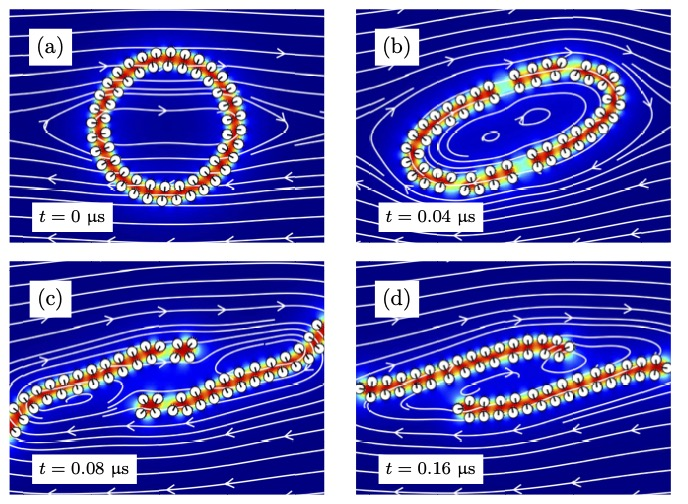
\includegraphics[width=0.475\textwidth]{figures/PreliminaryWork/Rupture.jpg}
\caption{\label{fig:JPv_rupture} \footnotesize Rupture of a granular
  vesicle under large shear rates.}
\end{wrapfigure}

In terms of hydrodynamics, the granule vesicles in background flows
replicate the behaviour of a continuous, permeable, inextensible,
elastic vesicle. The simulations showed, for the first time, a
granule-vesicle suspension behaving as a tank-treading
vesicle~\cite{Finken2008, Shaqfeh11} (see
Figure~\ref{fig:JPv_linearshear}). Movies of
Figure~\ref{fig:JPv_linearshear} reveal intermonolayer slip and derived
values for intermonolayer friction are in good quantitative agreement
those derived by atomistic and Martini force field simulation
studies~\cite{WuoEd06, denOtter2007, SHKULIPA2005823, Zgorski2019}. In
Figure~\ref{fig:JPv_rupture}, membrane rupture occurs at large shear
rates and yields a dimensional scaling for critical rupture shear
rate~\cite{VLAHOVSKA2009775, keller_skalak_1982}. A side-by-side
comparison of granule-based vesicles and the sharp interface
representation yields shapes and trajectories that basically overlapped.

%Having a non-specific model that replicates physical details
%is the crown jewel of applied mathematics.
The mathematical framework in
equations~\eqref{eq:RBT}--\eqref{eqn:stressbalance} is highly desirable
from the Applied Math point of view as there are many \emph{Further
Applications}, such as (i) amphiphilic Janus spheres that form diverse
suprastructures~\cite{HaBr20, McBr21, Bradley2017}, (ii) pickering
emulsions involving two-phase fluids and dense suspensions
\cite{Bradley2016}, (iii) creation and manipulation of small droplets
using amphiphilic microparticles~\cite{Ha2022SurfaceEM,
Ha2020MinimalSC}, and (iv) tension driven fabrication of
microstructures~\cite{Dasgupta2017, Leong2007, Reynolds2019, Cho2010,
Zeng20223DprintedMT, Russell2016EnergyLF}.

\subsection{Computational method and mathematical properties}
\begin{wrapfigure}[17]{r}{3.1in}
  \vspace{-8pt}
  \centering
  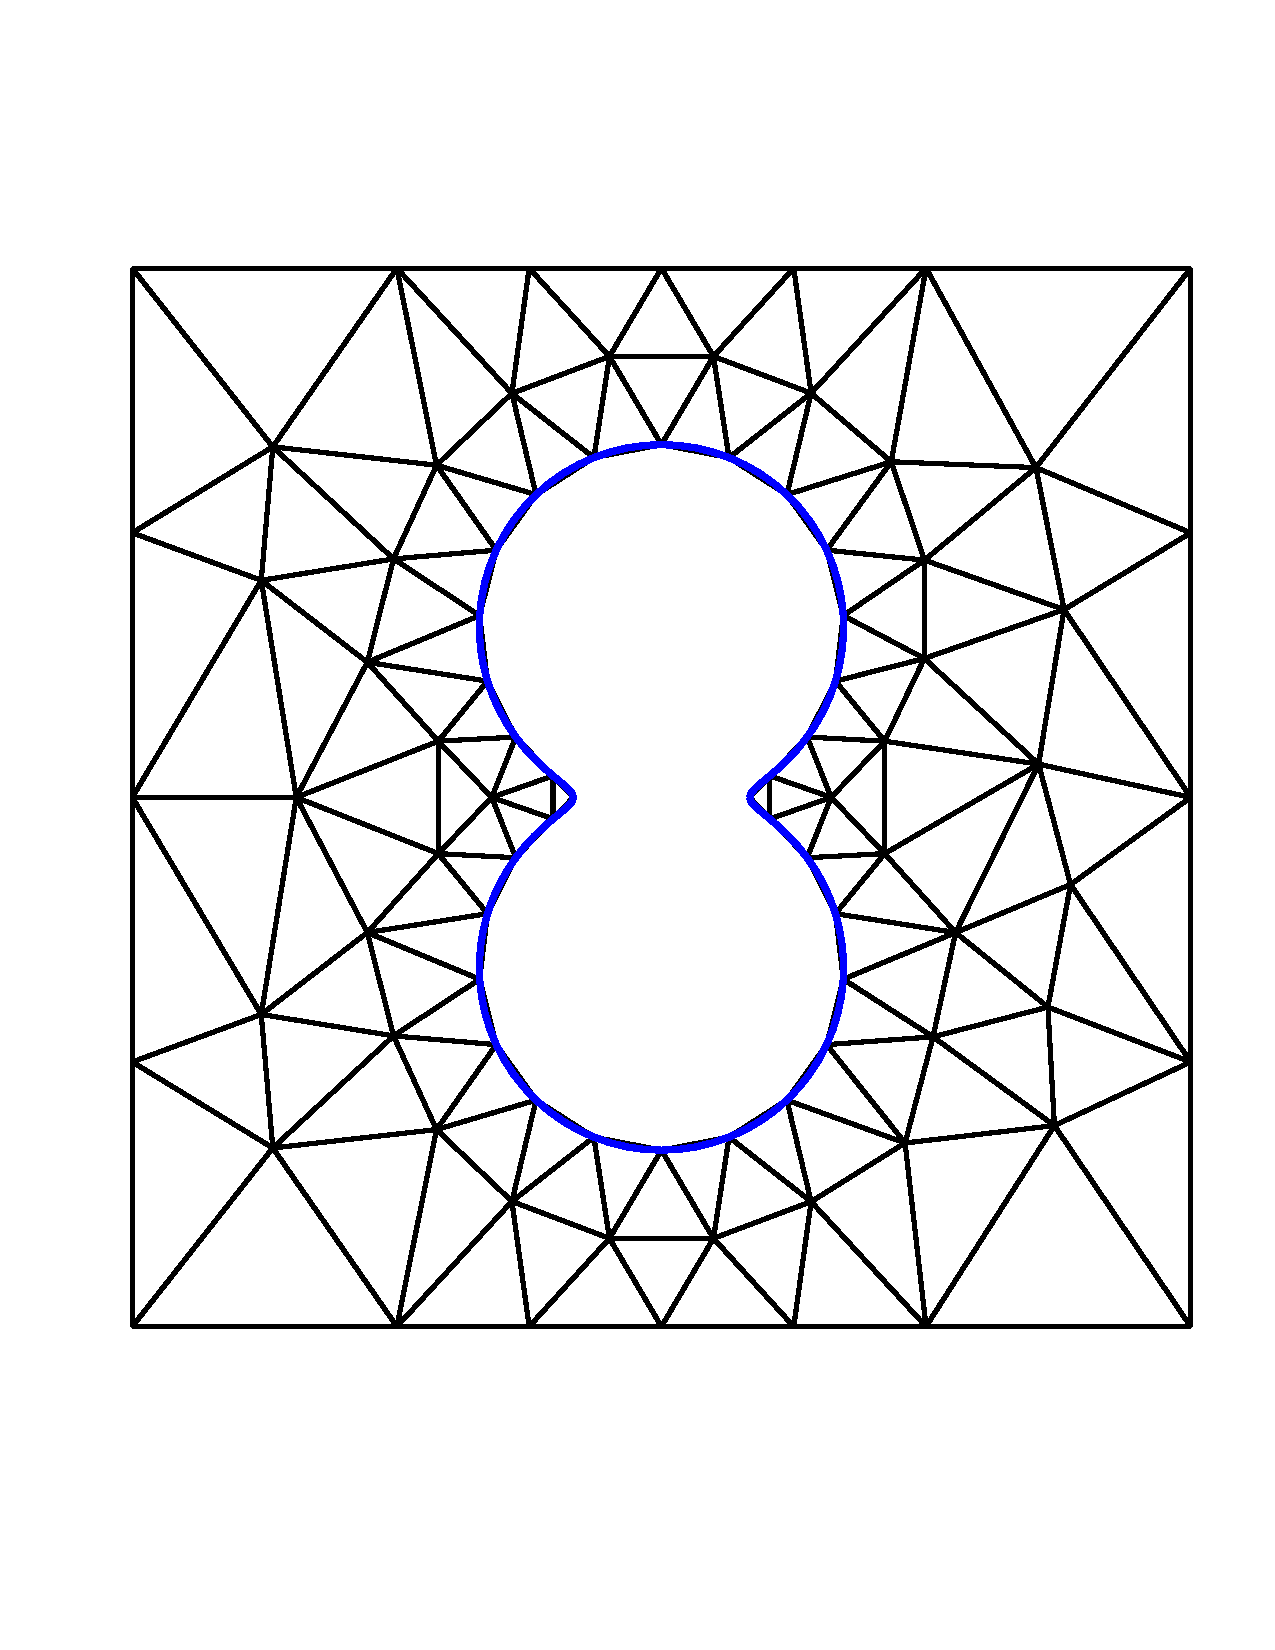
\includegraphics[width=1.5in]{figures/Background/Peanut/PeanutFEM.pdf}
  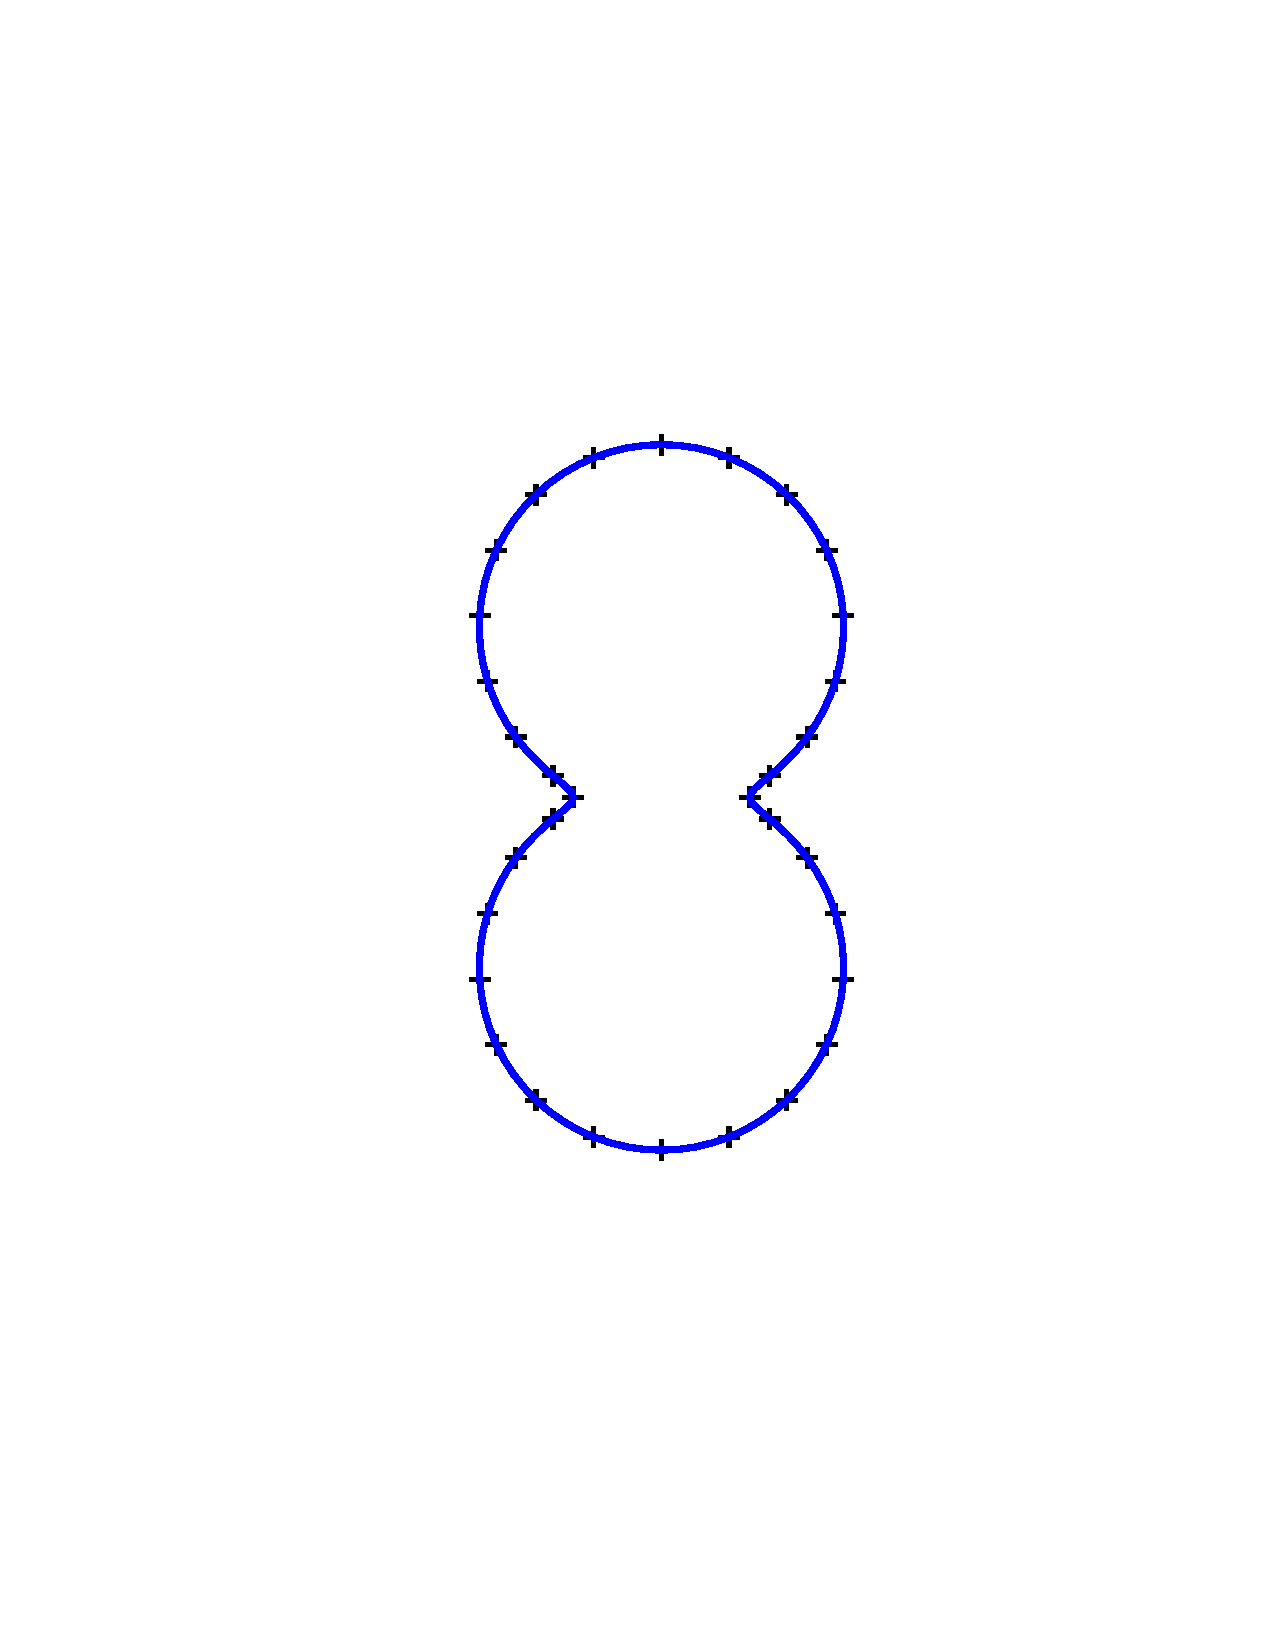
\includegraphics[width=1.5in]{figures/Background/Peanut/PeanutIE.pdf}\\
  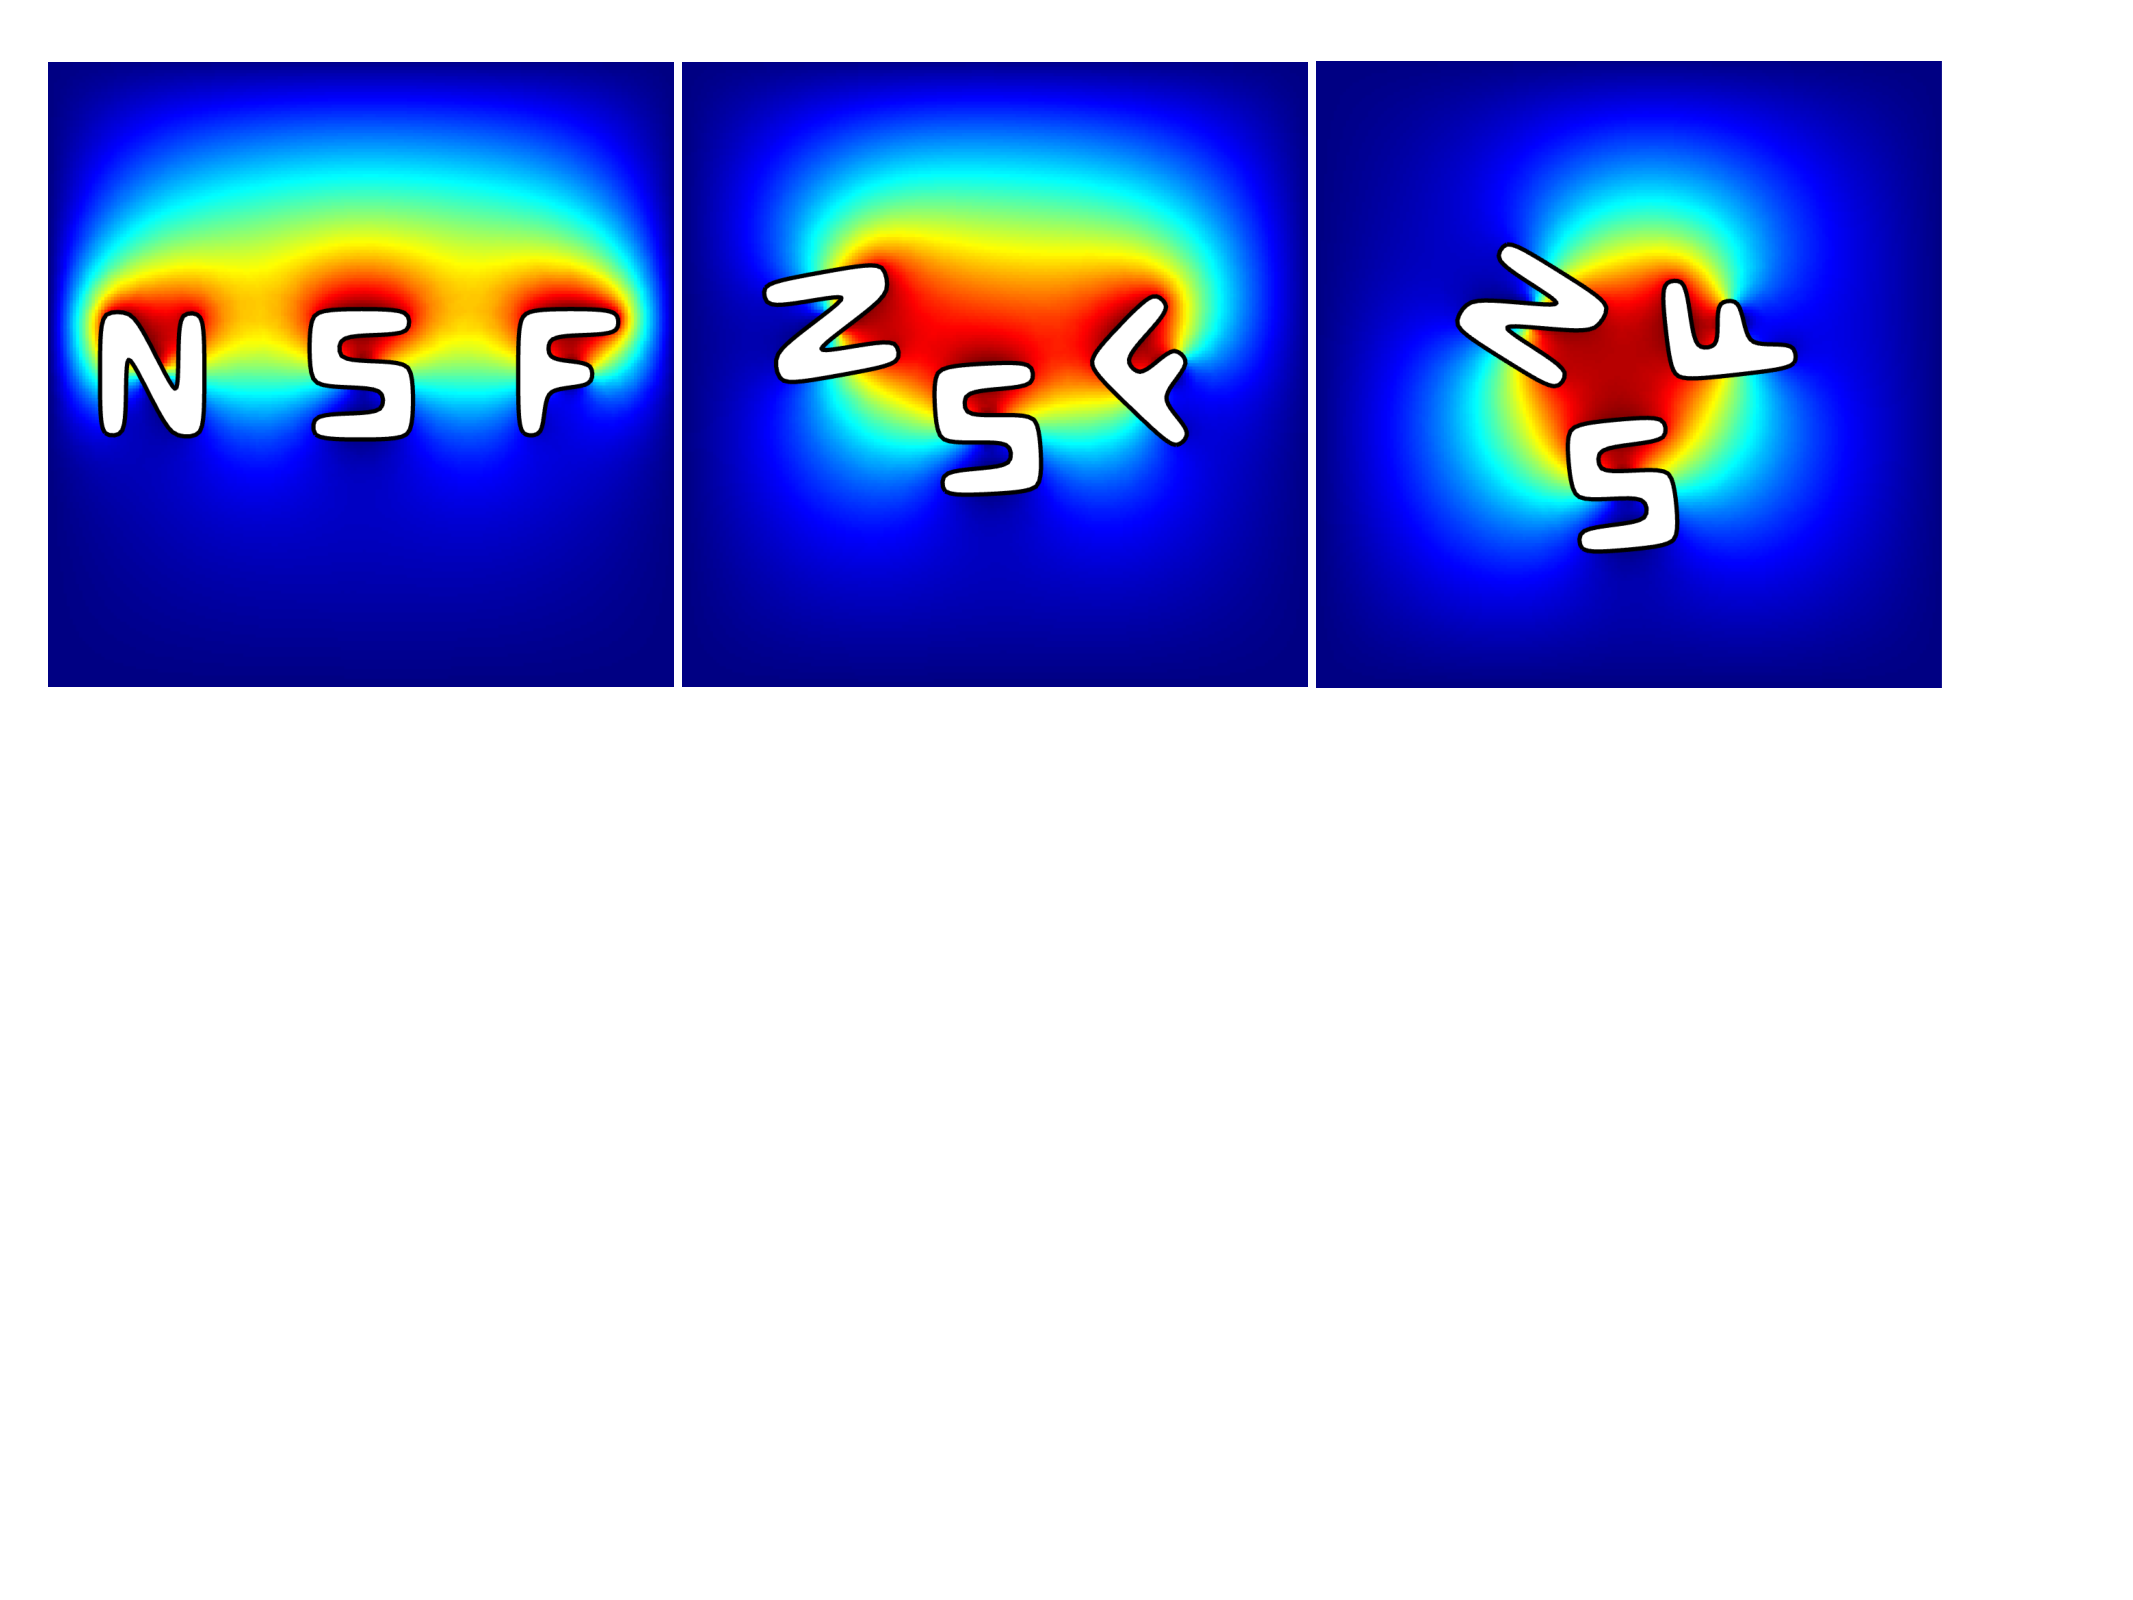
\includegraphics[width=3in]{figures/Background/NSF.pdf}\\
\caption{\label{fig:fem_vs_bie} \footnotesize A finite element method
  ({\em top left}) requires meshing the entire domain (typically into
  triangles), while a BIE ({\em top right}) requires meshing only the
  boundary of the domain.
  ({\em bottom}) BIE can handle intricately shaped domains as well.}
\end{wrapfigure}
Computational methods to solve the partial differential equations
(PDEs)~\eqref{eqn:stokes} and~\eqref{eqn:phase} are challenging to
develop because of the complicated and unbounded domain. This challenge
is compounded when dense suspensions are considered.
Integral equations
(IEs) offer an alternative formulation of the PDEs that only require
meshing the boundary of the granules rather than all of $\Omega(t)$
(Figure~\ref{fig:fem_vs_bie}), and they automatically satisfy far-field
conditions. Additional advantages of discretizations of IE formulations
include high-order, or even spectral, accuracy and well-conditioned
linear system that can be solved iteratively with a mesh-independent
number of Krylov iterations such as the generalized minimal residual
method (GMRES). However, IEs have challenges: nearly touching granules
requires a quadrature rule for nearly-singular integrals; their
discretization results in dense matrices; and they cannot immediately be
applied to non-linear PDEs. \S\ref{sec:specificaim2} discusses a variety
of tools the IE community, including PI Quaife, has developed to address
these numerical challenges.

In the absence of external flow, the
system~\eqref{eq:RBT}--\eqref{eqn:stressbalance} has the energy law
\begin{align}
\label{eq:energy_law}
  \frac{d}{dt}E
  = - \int_{\Omega(t)}\tfrac{1}{2}\mu|\nabla \uu + \nabla
  \uu^T|^2 \,d\xx,\quad
    E = \gamma \int_{\Omega(t)}
  \frac{\epsilon}{2} |\nabla \phi|^2 + \frac{1}{\epsilon} W(\phi) \,d\xx.
\end{align}
Here $E$ is the energy stored by solvent phase transitions to the
boundary. It states that energy is always lost as viscous
dissipation. The derivation of~\eqref{eq:energy_law} is interesting
because $E$ depends both on $\phi$ and $\Omega(t)$. It uses the Rayleigh
Transport Theorem to write the time derivative of $E$ as an energy
density flux through the boundary involving the phase stress $T_i$, and
a bulk term involving the Euler-Lagrange derivative of
$E$~\cite{Fu2018_SIAM}. The Euler-Lagrange derivative vanishes due
to~\eqref{eqn:phase} and the boundary flux transforms into viscous
dissipation due to~\eqref{eqn:hydro_stress} and the Stokes equations.
Furthermore, the integral of the phase stress vectors $T_i\nnu$ over
$\partial \Omega$ is zero. Figure~\ref{fig:coarsening} summarizes the
general evolution of $E$ from the self-assembly process to the
collective dynamics of the assembly under external forcing.


\begin{wrapfigure}[16]{r}{4in} 
  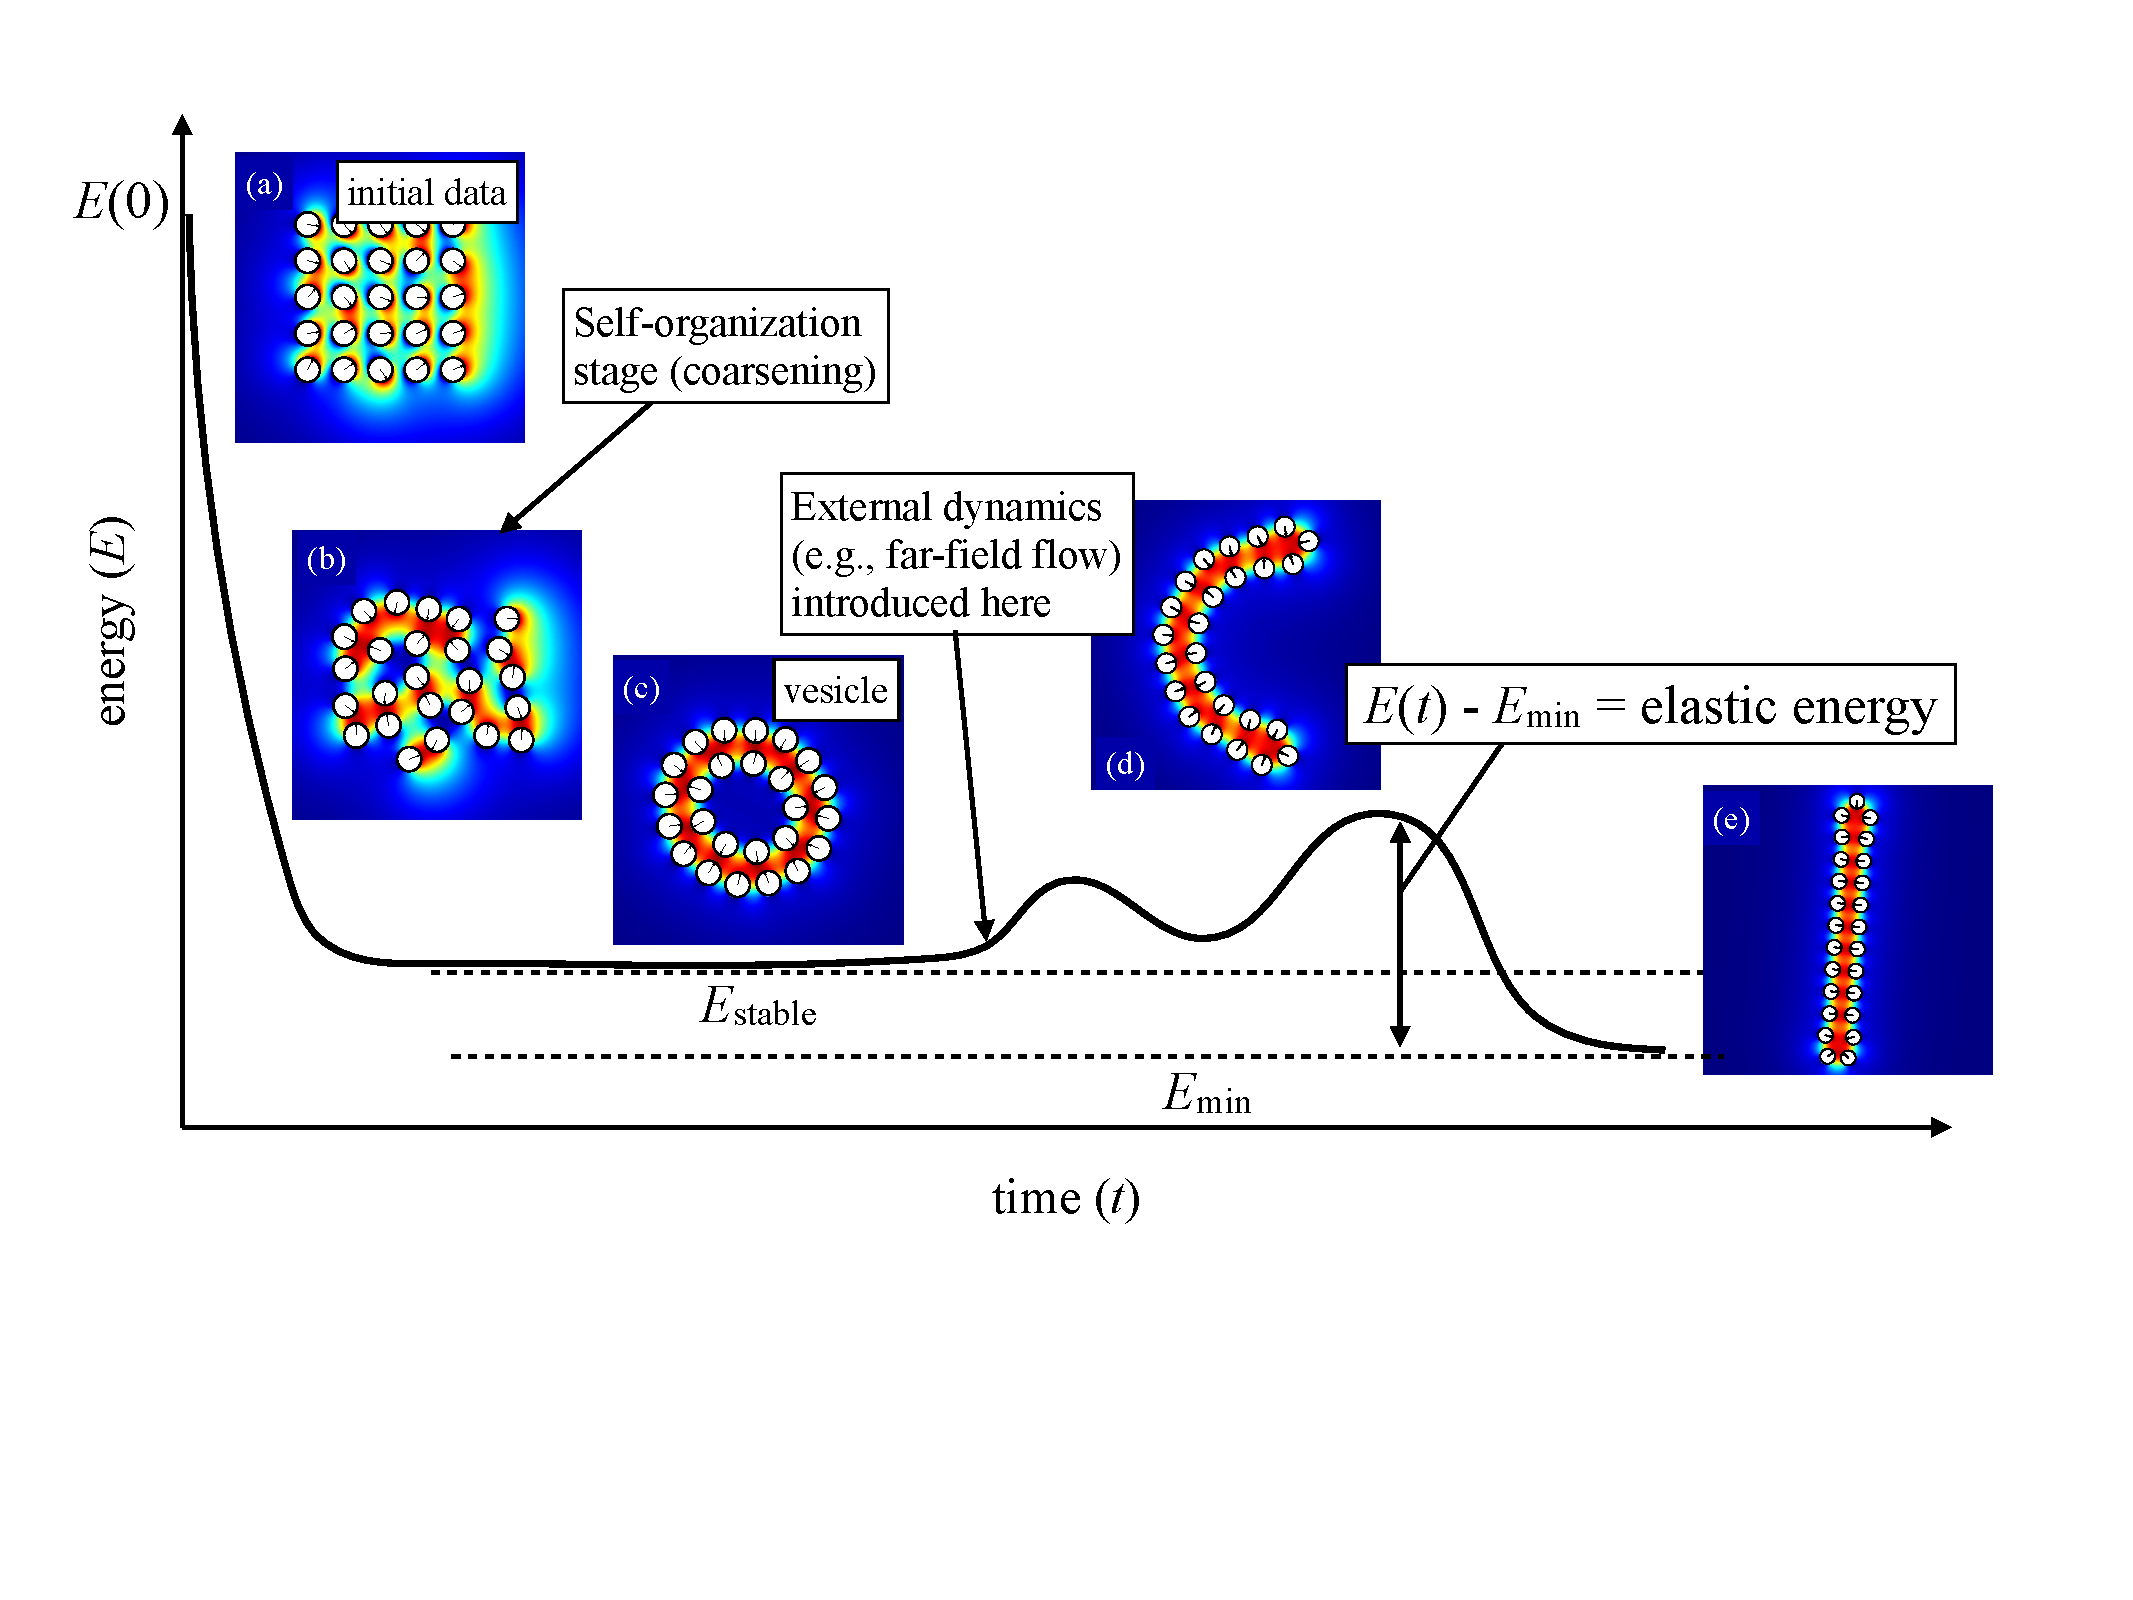
\includegraphics[width=4in]{figures/Background/coarsening.pdf}
  \vspace{-25pt}
  \caption{\label{fig:coarsening} \footnotesize Energy $E$ in
  equation~(\ref{eq:energy_law}) of a suspension of amphiphilic granules
  versus time $t$. Under the moving domain problem
  \eqref{eq:RBT}--\eqref{eqn:hydro_stress} with amphiphilic boundary
  condition, the granules self-organize into vesicle bilayers. External
  hydrodynamic effects are introduced to study elastic properties of
  the granules assembly~\cite{Fu2018_SIAM,FuQuRyYo22}.}
\end{wrapfigure}

We have $\lim_{\xx \to \infty} \phi(\xx) = \phi_0$ in the far field and
when background flows are involved, we require that $\lim_{\xx \to
\infty} \uu(\xx) - \uu_{\infty}(\xx) = \mathbf{0}$, where $\uu_{\infty}$
can take the form
%In the case of shear background flow,
%for example,
%\begin{align}
%\label{eqn:shear_BG_flow}
%\uu_{\infty}(\xx) = \dot{\gamma} \xx \cdot \mathbf{e}_y \mathbf{e}_x,
%\end{align}
%where $\dot \gamma$ is the shear rate and $\mathbf{e}_x$, $\mathbf{e}_y$
%are horizontal and vertical basis vectors, respectively.
%Other
%background flows include
of a shear, extensional, parabolic Poiseuille, or Taylor-Green flow, for
example. For numerical stability, we include pairwise repulsive forces
and torques in~\eqref{eqn:stressbalance} to prevent the near-collision
between neighboring granules. This introduces a repulsive potential in
the energy law~\eqref{eq:energy_law}. Background flow adds elastic
energy to the granule configurations, as illustrated in
Figure~\ref{fig:coarsening}.
%and is quantified by simulation. We refer to the
%PIs work~\cite{FuQuRyYo22, fu-ryh-qua-you2022, Fu2018_SIAM} for details. 

In terms of physical justification, the derivation of the
one-dimensional version of our model was carried out using a Landau
expansion for a single-well potential~\cite{MaRa76, ErLjCl89}.
The double-well potential case was
considered by Gompper~\cite{GoHaKo94} to describe metastable
coordination of water. In the field of surface
chemistry~\cite{Israelachvili1954}, there is a large empirical
literature on properties of long-range hydrophobic
interaction~\cite{LeRaPa77, KoNa15, Nagle17, Lum1999, Lin2005,
Meyer2006, Ducker2016, Jackson2016, Gletal88, Aketal17, Ch05}. The
stress~\eqref{eqn:stressbalance} was first identified by PIs Ryham and
Young in~\cite{Fu2018_SIAM} and generalizes one-dimensional hydrophobic
interaction to the $n$-dimensional setting. 

Regarding the mathematical motivation for~\eqref{eq:RBT}--\eqref{eqn:stressbalance},
when equation \eqref{eqn:phase} takes the form of a screened Laplace equation
$-\epsilon^2 \Delta \phi + \phi =0$, for a fixed domain $\Omega$ with
smooth boundary, if the material label $h_i = 1$
everywhere, then $\phi$ has a boundary layer going from $1$ at the
boundary to $0$ so that 
$\lim_{\epsilon \to 0} E = \frac{1}{2}\gamma |\partial \Omega|$.
In other words, 
interfacial energy enters the problem even in the linear case,
\emph{because of the introduction of granule boundaries.}
We are confident
that~\eqref{eq:RBT}--\eqref{eqn:stressbalance} is a correct description
of long-range interactions between granule surfaces.


\subsection{Outline of the proposal}
The aim of this proposal is to advance the simulation and theory for
soft-matter systems and foster training in Mathematical Sciences.
Section~\ref{sec:BroaderImpacts} summarizes the broader impacts and
section~\ref{sec:IntellectualMerit} summarizes the intellectual merit of
our research activity. Section~\ref{sec:proposed-work} contains our
specific aims.




